% !Mode::"TeX:UTF-8"

% -------------------- Information --------------------

\newcommand{\TITLE}{求解偏微分方程的有限元方法}
\newcommand{\AUTHOR}{Jason}
\newcommand{\SUBJECT}{偏微分方程数值解}
\newcommand{\KEYWORDS}{}

% -------------------- Packages --------------------

\documentclass[a4paper, 12pt]{ctexart}
\usepackage{amsmath}
\usepackage{amssymb}
% \usepackage{amsthm} % 定理格式 由ntheorem代替.
\usepackage{authblk} % 作者 (见校赛论文).
\usepackage{array}
\usepackage{bigfoot} % to allow verbatim in footnote.
\usepackage{bm} % \bm for bold symbols.
\usepackage{boldline} % 长表格表格线加粗.
\usepackage{caption} % 题注.
\usepackage{commath} % abs, norm
\usepackage{enumerate}
% \usepackage{enumitem} 用enumerate包代替.
\usepackage{fancyhdr} % 脚注.
\usepackage{filecontents}
\usepackage{flafter} % 不让float出现在定义之前的地方.
\usepackage{float} % 你们这帮float给我乖乖听话 HHHHHHHHHHH.
\usepackage[T1]{fontenc} % Bera Mono Font
\usepackage{fontspec} % 字体.
\usepackage{graphicx}
\usepackage{hyperref}
\usepackage{lastpage}
\usepackage{letltxmacro} % \let
\usepackage{lipsum}
\usepackage{listings} % 排版程序语言.
\usepackage{longtable} % 长表格.
\usepackage{makecell} % 表格线加粗 \Xhline{1.2pt}.
\usepackage{mathtools} % \xleftrightarrow.
\usepackage{mathrsfs} % \mathscr
\usepackage{multirow} % 合并单元格.
\usepackage[square, numbers, sort&compress]{natbib} % 引用.
\usepackage[thmmarks, amsmath, thref]{ntheorem} % 定理格式.
\usepackage[section]{placeins} % 使图像不会显示在别的部分 若过于严格则换成[below].
\usepackage{stackrel} % 上下写 见校赛论文.
\usepackage{subcaption} % subcaption and subfigure
% \usepackage{SUBSubsubsection}
\usepackage{titlesec} % Section标题格式.
\usepackage{varioref} % For Cross References.
\usepackage[dvipsnames]{xcolor} % 颜色声明.
\usepackage{xfrac} %\sfrac{}{}
\usepackage[all, cmtip]{xy} % Commutive diagram.

% Require `ntheorem'

\usepackage[mathlines, edtable]{lineno} % Line numbers.
    %\begin{edtable}{tabular}[<args>] <entries> \end{edtable}

% Require `xcolor'

\usepackage[numbered, framed]{matlab-prettifier}
\usepackage{pgfplots}
\usepackage{pgfplotstable}
\usepackage{tikz}

% Incompatible with `matlab-prettifier'

\usepackage[printwatermark]{xwatermark} % Foreground Watermarks.

% -------------------- Settings --------------------

% Title

\title{\TITLE}
\author{\AUTHOR}
\date{\today}

% Package: caption

\captionsetup{
    margin    =   6pt,
    font      =   small,
    labelfont =   bf
}

% Package: ctex

\setCJKfamilyfont{fzstk}{FZShuTi} % 方正舒体
\newcommand{\fzstk}{\CJKfamily{fzstk}}

% Package: fancyhdr

\setlength{\headheight}{15pt}
\lhead{Copyright \copyright\ \AUTHOR}
\rhead{Page \thepage\ of \pageref{LastPage}}

% Package: graphicx

\graphicspath{{resources/}} % 图像文件目录

% Package: hyperref

\hypersetup{
    linktoc             =   all,
    colorlinks          =   true,
    linkcolor           =   cyan,
    anchorcolor         =   black,
    citecolor           =   green,
    filecolor           =   cyan,
    menucolor           =   red,
    runcolor            =   filecolor,
    urlcolor            =   magenta,
	pdftitle           	=   {\TITLE},
	pdfauthor          	=   {\AUTHOR},
	pdfsubject         	=   {\SUBJECT},
	pdfcreator			=	{Visual Studio Code},
	pdfproducer			=	{XeLaTeX with documentclass ctexart},
	pdfkeywords        	=   {\KEYWORDS},
    bookmarksnumbered   =   true,
    pdfstartview        =   FitH,
    pdfpagelayout       =   OneColumn
}

% Package: lineno

\renewcommand{\linenumberfont}{\normalfont\scriptsize\sffamily}

\let\oldlstinputlisting\lstinputlisting
\renewcommand{\lstinputlisting}[2][\empty]{
    \par\nolinenumbers\oldlstinputlisting[#1]{#2}\linenumbers\par
}

\let\oldlstlisting\lstlisting
\let\oldendlstlisting\endlstlisting
\renewenvironment{lstlisting}
    {\par\nolinenumbers\oldlstlisting}
    {\oldendlstlisting\endnolinenumbers\par}

\let\oldtable\table
\let\oldendtable\endtable
\renewenvironment{table}
    {\par\nolinenumbers\oldtable}
    {\oldendtable\endnolinenumbers\par}

% Package: listings

%% Title

\renewcommand\lstlistingname{代码}
\renewcommand\lstlistlistingname{代码}

%% Lstinline with color box

\LetLtxMacro{\oldlstinline}{\lstinline}
\renewcommand{\lstinline}[2][]{\colorbox{lightgray}{\oldlstinline[#1]{#2}}}
\newcommand{\matlabinline}[1]{
    \lstinline[style=MATLAB-editor, basicstyle=\mlttfamily]{#1}}

\lstset{
    breaklines=true,
    backgroundcolor=\color{lightgray},
    basicstyle=\scriptsize,
    inputpath=resources/,
    numbers=left,
    numberstyle={\color{black!33}\scriptsize\sffamily},
    xleftmargin=2em,
    xrightmargin=2em
}

% Package: ntheorem

%% Theorem
\newtheorem{theorem}{Theorem}[section]
\newtheorem{lemma}[theorem]{Lemma}
\newtheorem{corollary}[theorem]{Corollary}
%% Problem
\theoremstyle{plain}
\newtheorem{problem}{Problem}[section]
%% Proposition
\newtheorem{proposition}{Proposition}[section]
%% Conjecture
\newtheorem{conjecture}[proposition]{Conjecture}
%% Definition
\theoremstyle{plain}
\theoremheaderfont{\bfseries}
\theorembodyfont{\rmfamily}
\newtheorem{definition}{Definition}[section]
%% Note
\theoremstyle{plain}
\theoremheaderfont{\itshape}
\theorembodyfont{\itshape}
\newtheorem{note}{Note}[section]
%% Proof
\theoremstyle{nonumberplain}
\theoremheaderfont{\itshape}
\theorembodyfont{\upshape}
\theoremseparator{.}
\theoremsymbol{\ensuremath{\square}}
\newtheorem{proof}{Proof}
%% Solution
\theoremsymbol{\ensuremath{\blacksquare}}
\newtheorem{solution}{Solution}

% Package: pgfplots

\pgfplotsset{width=7cm, compat=1.16}

% Package: pgfplotstable

\pgfplotstableset{
    every head row/.style={before row=\Xhline{1.2pt},after row=\hline},
    every last row/.style={after row=\Xhline{1.2pt}}
}

% Package: varioref

\renewcommand{\reftextbefore}
    {on the \reftextvario{preceding page}{page before}}
\renewcommand{\reftextafter}
    {on the \reftextvario{following}{next} page}
\renewcommand{\reftextfacebefore}
    {on the \reftextvario{facing}{preceding} page}
\renewcommand{\reftextfaceafter}
    {on the \reftextvario{facing}{next} page}
\renewcommand{\reftextfaraway}[1]
    {on page \pageref{#1}}

%% Label formats

\labelformat{lstlisting}{代码#1}
\labelformat{equation}{式(#1)}
\labelformat{figure}{图#1}
\labelformat{table}{表#1}
\labelformat{problem}{Problem #1}

% Package: xwatermark

\newsavebox\mybox
\savebox\mybox{\tikz[color=cyan, opacity=0.2]\node{\fzstk\SUBJECT};}
\newwatermark*[
    allpages,
    angle=45,
    scale=6,
    xpos=-20,
    ypos=15
]{\usebox\mybox}

% -------------------- General new commands --------------------

\DeclareMathAlphabet{\mathsfsl}{OT1}{cmss}{m}{sl}

\DeclareMathOperator{\arcosh}{arcosh}
\DeclareMathOperator{\Arcosh}{Arcosh}
\DeclareMathOperator*{\Beta}{B}
\DeclareMathOperator{\Log}{Log}
\DeclareMathOperator*{\real}{Re}
\DeclareMathOperator*{\image}{Im}

% Expectation

\newcommand{\expect}{\operatorname{E}\expectarg}
\DeclarePairedDelimiterX{\expectarg}[1]{(}{)}{
    \ifnum\currentgrouptype=16 \else\begingroup\fi
    \activatebar#1
    \ifnum\currentgrouptype=16 \else\endgroup\fi
}

\newcommand{\innermid}{\nonscript\;\delimsize\vert\nonscript\;}
\newcommand{\activatebar}{
    \begingroup\lccode`\~=`\|
    \lowercase{\endgroup\let~}\innermid
    \mathcode`|=\string"8000
}

\newcommand*{\BC}{\mathbb{C}}
\newcommand*{\BR}{\mathbb{R}}
\newcommand*{\diff}{\mathop{}\!\mathrm{d}}
\newcommand*{\matr}[1]{\ensuremath{\mathsfsl{#1}}} % italic sans serif
\newcommand*{\me}{\mathrm{e}}
\newcommand*{\mi}{\mathrm{i}}
\newcommand*{\restrict}[1]{\raisebox{-.5ex}{$\vert$}_{#1}}
\newcommand*{\vect}[1]{\bm{#1}}

% -------------------- Specific new commands --------------------



% -------------------- Document --------------------

\begin{document}

    % -------------------- Title Page --------------------

    \maketitle
    \thispagestyle{empty}
    \pagenumbering{roman}

    % -------------------- Abstract Page --------------------

    % -------------------- Contents --------------------

    % \newpage
    % \tableofcontents

    % -------------------- Body --------------------

    \newpage
    \pagestyle{fancy}
    \pagenumbering{arabic}
    \linenumbers

    \section{知识点整理}

    在新版本MATLAB下函数\matlabinline{initmesh}和\matlabinline{assempde}, 取而代之的是函数\matlabinline{generateMesh}和\matlabinline{solvepde}与以\matlabinline{model}变量为核心的编程思路. 接下来我们整理一下求解偏微分方程数值解的流程.

    \begin{enumerate}[Step 1.]
        \item 用\matlabinline{createpde}函数生成\matlabinline{model}变量.
        \item 用\matlabinline{decsg}函数生成方程的分解几何矩阵.
        \item 用\matlabinline{geometryFromEdges}函数将分解几何矩阵添加进\matlabinline{model}变量.
        \item 用\matlabinline{specifyCoefficients}函数确定方程中的参数.
        \item 用\matlabinline{setInitialConditions}函数添加初值条件.
        \item 用\matlabinline{applyBoundaryCondition}函数添加边值条件.
        \item 用\matlabinline{generateMesh}函数生成mesh.
        \item 用\matlabinline{solvepde}函数求出数值解.
    \end{enumerate}

    \section{问题与解答}

    \begin{problem}
        \label{problem: 1}
        求解以下边值问题:
        \begin{equation}
            \left\{
            \begin{aligned}
                &\Delta u-10u=f,\quad (x,y)\in\Omega,\\
                &u=0,\quad (x,y)\in\partial\Omega.
            \end{aligned}
            \right.
        \end{equation}
    \end{problem}

    \begin{solution}
        本题为Dirichlet边界条件的椭圆型偏微分方程.

        我们令$\mu$为单位圆盘$\mathbb{D}$, 记$E_{i}$表示第$i$象限, 则我们定义
        \begin{equation}
            f(x, y) = i,\quad (x, y)\in\Omega\cap E_{i},\quad i\in\mathbb{Z}_{4}.
        \end{equation}

        运行脚本可得如下图像:
        \begin{figure}[H]
            \centering
            \begin{subfigure}[b]{0.45\textwidth}
                \centering
                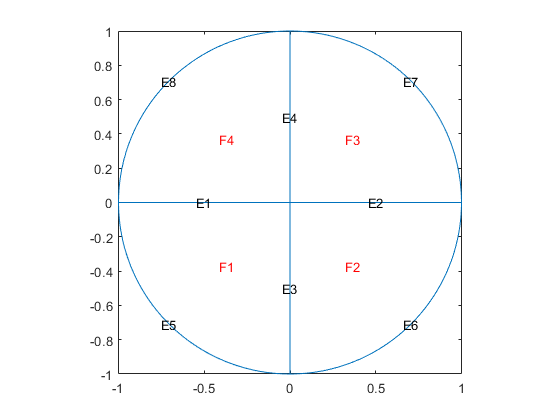
\includegraphics[width=\textwidth]{wc11.png}
                \caption{定义区域}
            \end{subfigure}
            \hfill
            \begin{subfigure}[b]{0.45\textwidth}
                \centering
                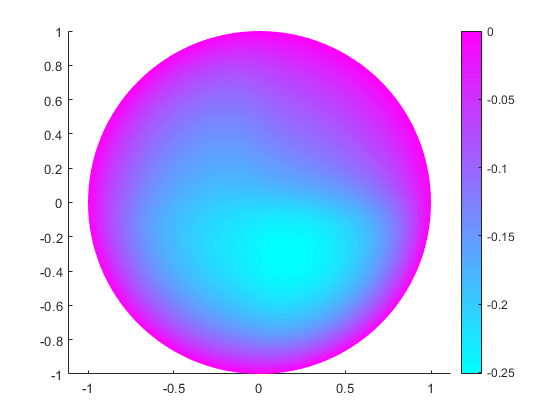
\includegraphics[width=\textwidth]{wc12.png}
                \caption{数值解}
            \end{subfigure}
            \caption{\ref{problem: 1}图像}
       \end{figure}

       可以看到尽管$f$在坐标轴上不连续, 但是得到的解的光滑性还是可以保证的.
    \end{solution}

    \begin{problem}
        \label{problem: 2}
        求解如下初边值问题:
        \begin{equation}
            \left\{
            \begin{aligned}
                &\frac{\partial u}{\partial t}-\frac{\partial^{2}u}{\partial x^{2}}-\frac{\partial^{2}u}{\partial y^{2}}=f(x,y,t),\quad (x,y,t)\in \Omega\times(0,1],\\
                &u(x,y,t)=xyt,\quad (x,y,t)\in\partial\Omega\times(0,1],\\
                &u(x,y,0)=0,\quad (x,y)\in\partial\Omega.
            \end{aligned}
            \right.
        \end{equation}
    \end{problem}

    \begin{solution}
        本题为Dirichlet边界条件的抛物型微分方程, 值得注意的是本方程与时间$t$有关.

        我们令$\Omega=\mathbb{D}$, 为了凸显与时间的相关性, 我们令$f$与$t$相关, 记
        \begin{equation}
            f(x,y,t) = x^{2}+y^{2}+t^{2}.
        \end{equation}

        运行脚本后所求得的解与时间$t$相关, 选取部分$t$的值, 绘得解的图像如下:
        \begin{figure}[H]
            \begin{subfigure}[b]{0.30\textwidth}
                \centering
                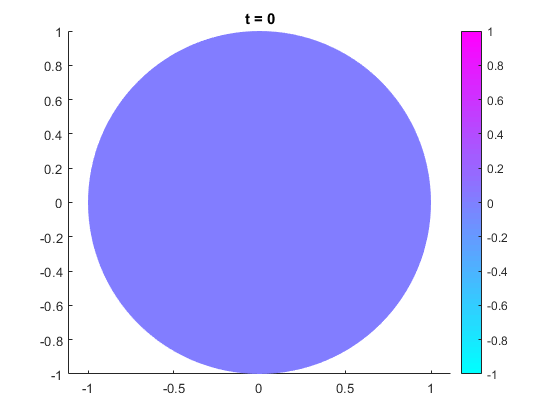
\includegraphics[width=\textwidth]{wc22.png}
                \caption{$u(x,y,0.0)$图像}
            \end{subfigure}
            \hfill
            \begin{subfigure}[b]{0.30\textwidth}
                \centering
                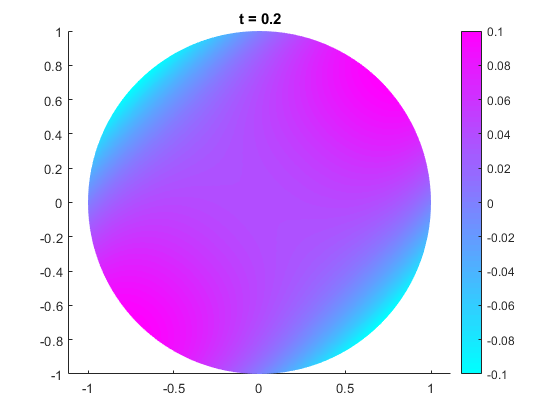
\includegraphics[width=\textwidth]{wc23.png}
                \caption{$u(x,y,0.2)$图像}
            \end{subfigure}
            \hfill
            \begin{subfigure}[b]{0.30\textwidth}
                \centering
                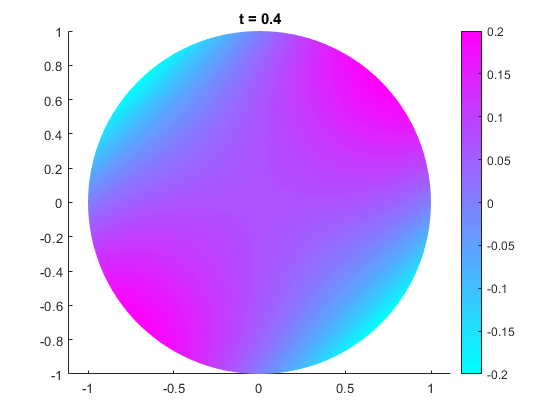
\includegraphics[width=\textwidth]{wc24.png}
                \caption{$u(x,y,0.4)$图像}
            \end{subfigure}
            
            \begin{subfigure}[b]{0.30\textwidth}
                \centering
                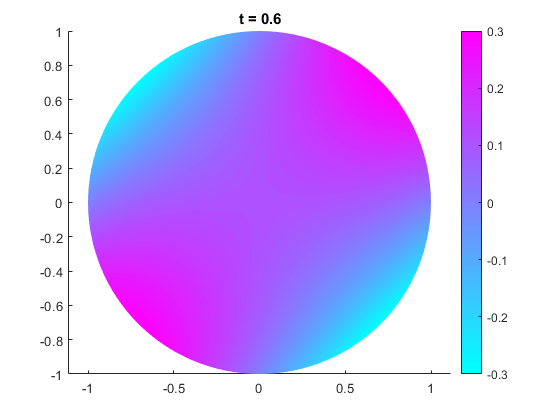
\includegraphics[width=\textwidth]{wc25.png}
                \caption{$u(x,y,0.6)$图像}
            \end{subfigure}
            \hfill
            \begin{subfigure}[b]{0.30\textwidth}
                \centering
                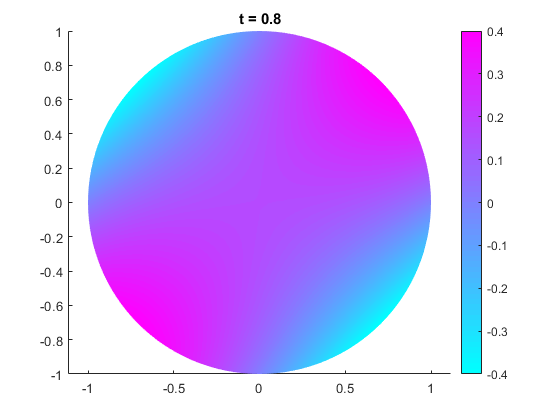
\includegraphics[width=\textwidth]{wc26.png}
                \caption{$u(x,y,0.8)$图像}
            \end{subfigure}
            \hfill
            \begin{subfigure}[b]{0.30\textwidth}
                \centering
                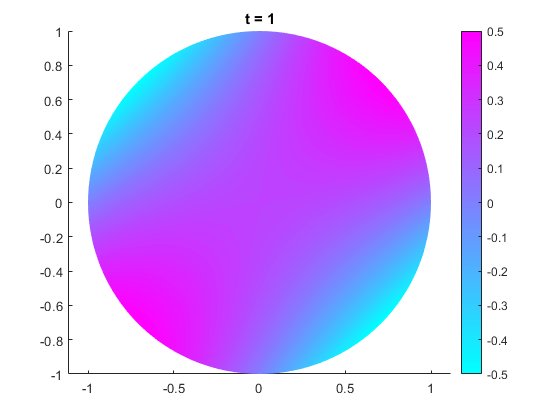
\includegraphics[width=\textwidth]{wc27.png}
                \caption{$u(x,y,1.0)$图像}
            \end{subfigure}
            \caption{\ref{problem: 2}图像}
        \end{figure}
    \end{solution}

    \begin{problem}
        \label{problem: 3}
        求解如下边值问题:
        \begin{equation}
            \left\{
            \begin{aligned}
                &-\frac{\partial^{2}u}{\partial x^{2}}-\frac{\partial^{2}u}{\partial y^{2}}=f(x,y),\quad (x,y)\in \Omega,\\
                &\frac{\partial u}{\partial n}+u^{3}=0,\quad (x,y)\in\partial\Omega.
            \end{aligned}
            \right.
        \end{equation}
    \end{problem}

    \begin{solution}
        这道题我们没能求得合适的结果.

        一开始我们绘制了两角形区域, 并取$f$为关于$x,y$的非线性函数, 发现算法并不收敛, MATLAB报错迭代超过次数. 于是我们尝试改进算法, 通过取$u^{[0]}=1$, 进行迭代来使边界条件线性化, 然而依旧得到了相同的错误. 最后我们简化问题, 令$f=g=1$, 区域$\Omega=\mathbb{D}$, 并绘制出此时Neumann边界条件的椭圆型方程的解, 得到结果为:
        \begin{figure}[H]
            \centering
            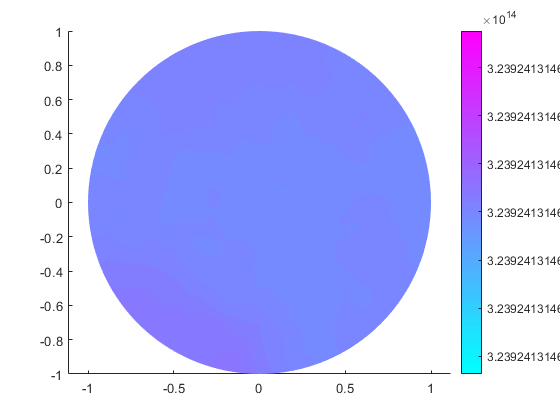
\includegraphics[width=0.45\textwidth]{wc31.png}
            \caption{\ref{problem: 3}失败集锦}
        \end{figure}
        可以看到解已经发散了.

        后续我们又调整了$u^{[0]}$, 令其即为$u$, 这样的话得到的$u^{[1]}$收敛. 但是利用$u^{[1]}$进行迭代时就又发散了. 我们找不出太好的办法来解决收敛性的问题.

        以下代码
        \begin{lstlisting}[
            caption=answer,
            style=MATLAB-editor,
            basicstyle=\mlttfamily\scriptsize,
            numberstyle={\color{black!33}\scriptsize\sffamily}
        ]
g = @(location, state) (-interpolateSolution(result, location.x, location.y).^3);
        \end{lstlisting}
        为迭代时$g$的更新定义, 通过用旧的解进行插值的方法估计非线性项, 以此线性化方程, 不知道写法是否有误.
    \end{solution}

    % -------------------- Bibliography --------------------

    % \newpage
    % \bibliography{Principles_of_Mathematical_Analysis}
    % \bibliographystyle{plain}

    % -------------------- Appendix --------------------

    \newpage
    \appendix

    \section{求解脚本}

    \subsection{\ref{problem: 1}}

    \lstinputlisting[
        caption=问题一求解脚本: wc3\_1.m,
        label={matlab: 1},
        style=MATLAB-editor,
        basicstyle=\mlttfamily\scriptsize
    ]{wc3_1.m}

    \subsection{\ref{problem: 2}}

    \lstinputlisting[
        caption=问题二求解脚本: wc3\_2.m,
        label={matlab: 2},
        style=MATLAB-editor,
        basicstyle=\mlttfamily\scriptsize
    ]{wc3_2.m}

    \subsection{\ref{problem: 3}}

    \lstinputlisting[
        caption=问题三尝试脚本: wc3\_3.m,
        label={matlab: 3},
        style=MATLAB-editor,
        basicstyle=\mlttfamily\scriptsize
    ]{wc3_3.m}
\end{document}
